\section{Results}

\subsection{Estimating coalescence times of alleles}

Figure \ref{fig:FC_Res_1} shows the distances calculated between the allelic pairs simulated from the ABC Iron Transporter and Large Ribosomal Subunit sequence pools, and between the allelic pairs identified from Fc Alleles RNAseq data.
The three distributions show considerable overlap, which implies that the divergence between allelic pairs identified from the genome is representative of the divergence between alleles from two known genes (Figure \ref{fig:FC_Res_1}).

\begin{figure}
\centering
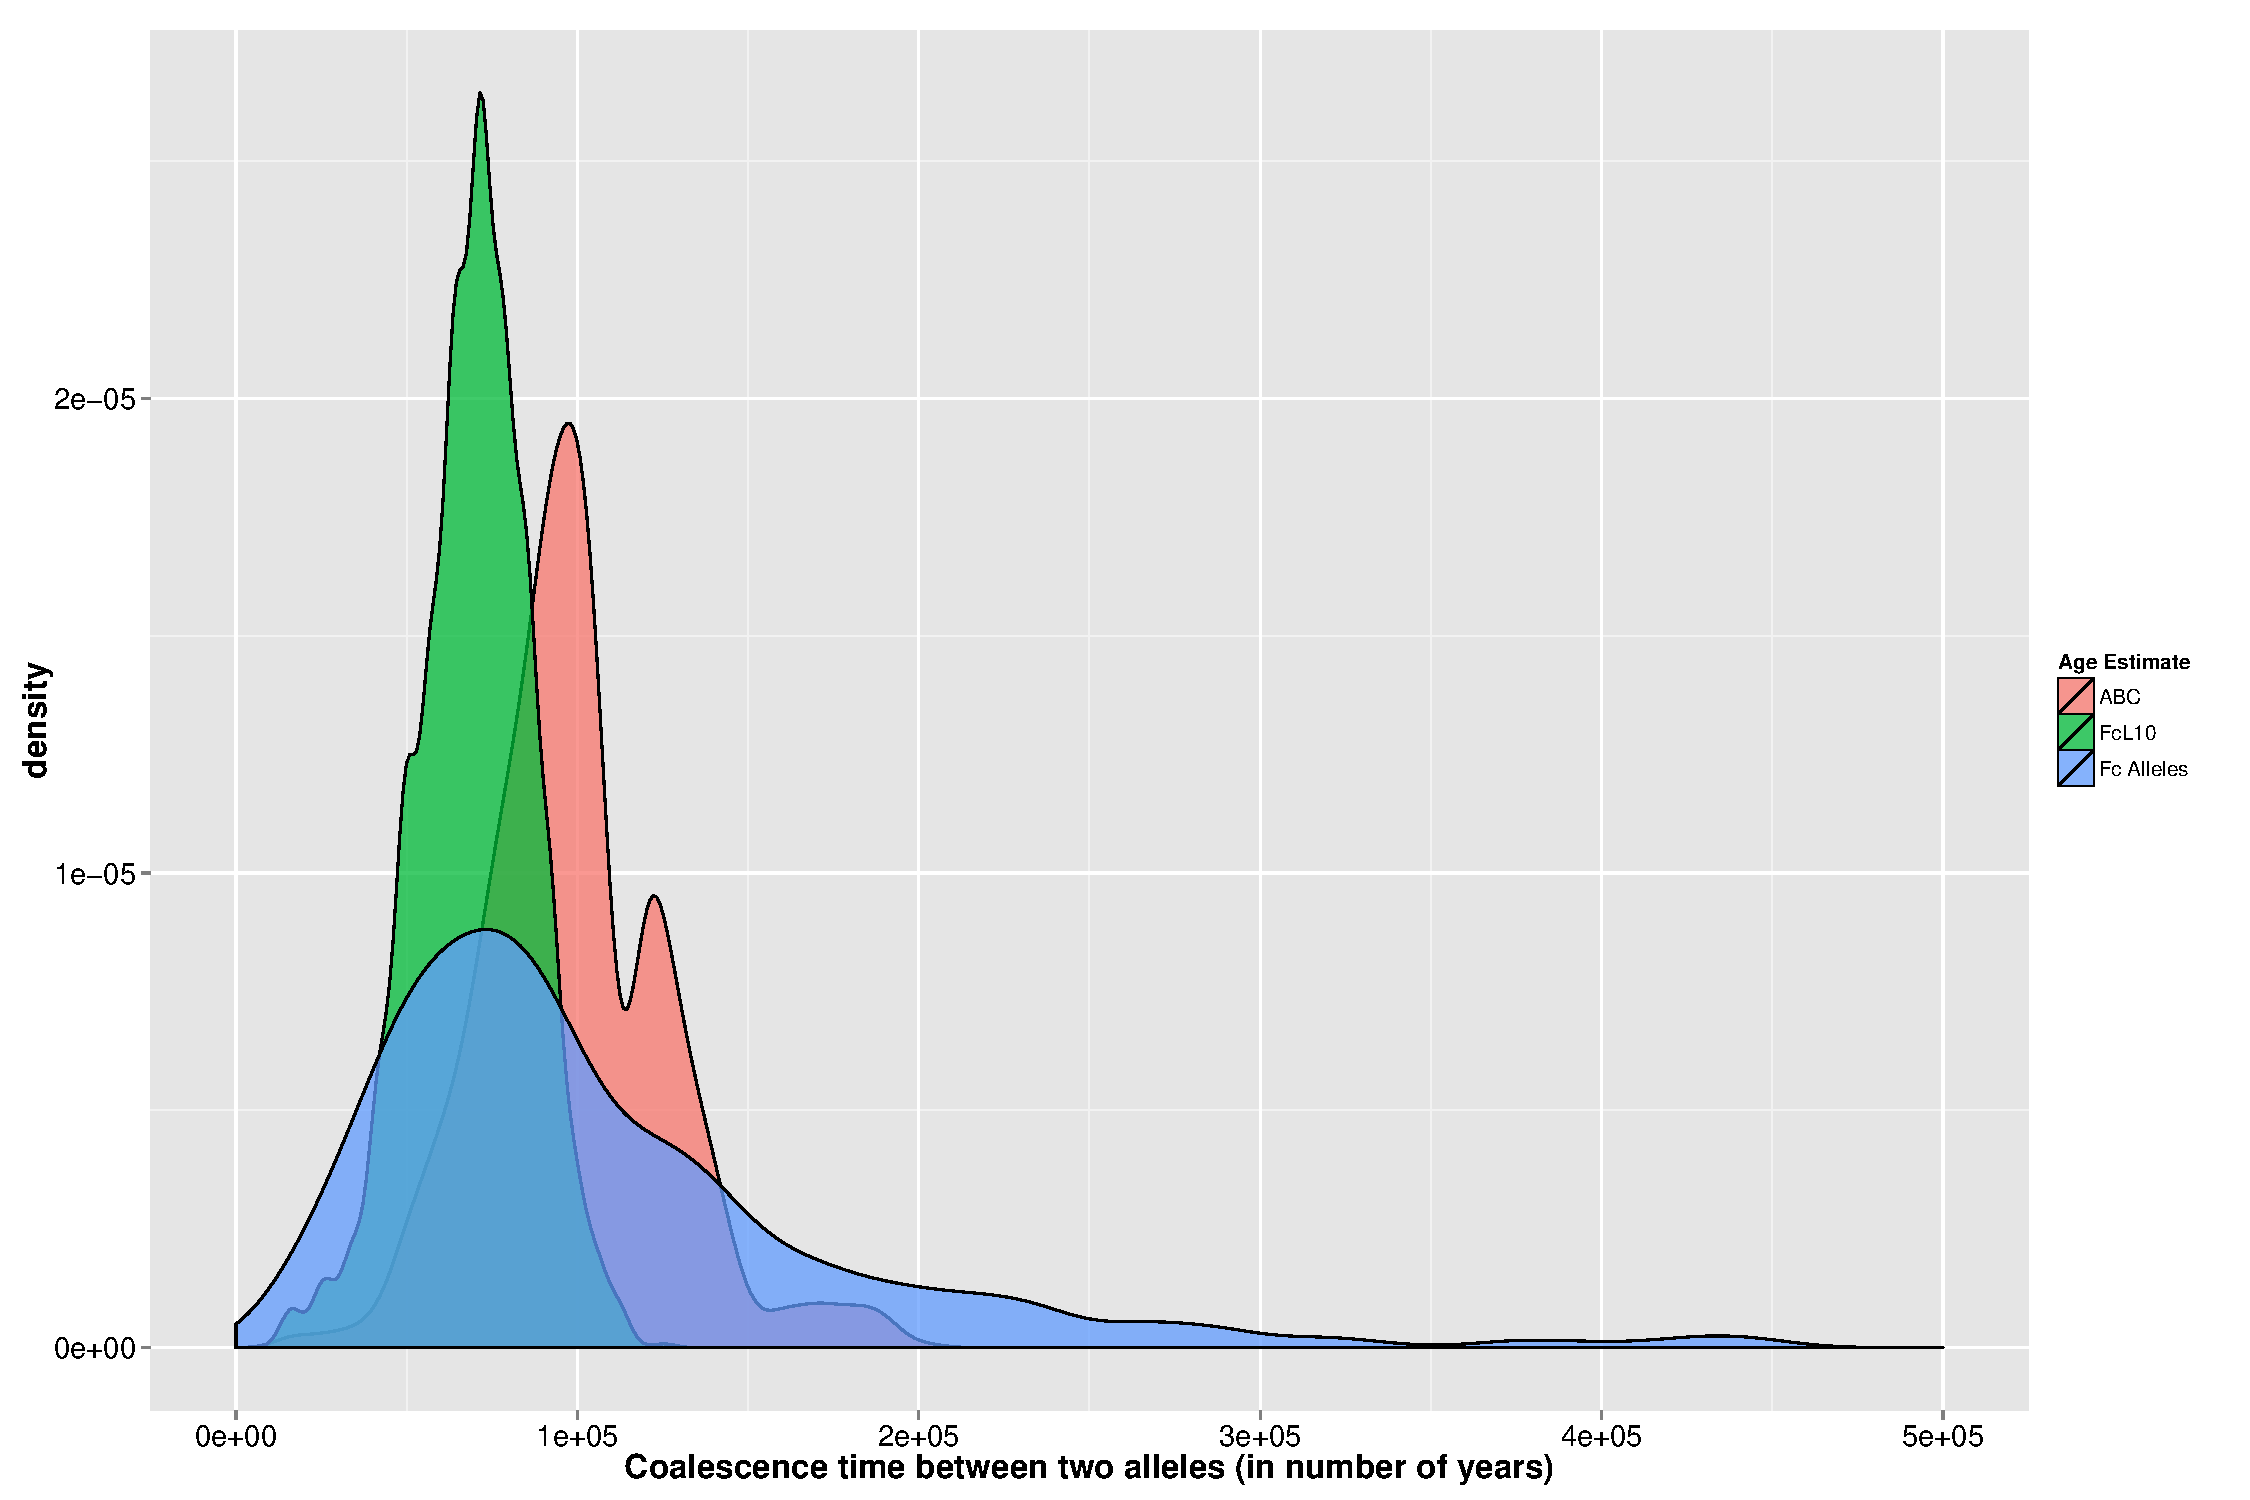
\includegraphics{Figures/Fcylindrus/DatesComparrisonMax}
\caption{Smoothed density plot of the maximum coalescence times (in generations) calculated for allelic pairs of the ABC Iron Transporter (red), Large Ribosomal Subunit (green) and allelic pairs from the genome (blue).\label{fig:FC_Res_1}}
\end{figure}

\subsection{Testing for recombination in the PCR amplified alleles with the PHI-test}

PHI – Scores calculated for the sequences of the ABC Iron transporter and the Large Ribosomal Subunit (Table \ref{table:Phitable}), and Figure \ref{fig:FC_Res_2} shows the refined incompatibility matrices between informative sites computed for the ABC Iron Transporter (A.), and the Large Ribosomal Subunit (B.). 
Yellow squares indicate pairs of informative sites that are compatible, darker squares indicate a pair of sites that are incompatible.
The presence of incompatible sites in these sequences, and the PHI-Scores and NSS scores shown in Table \ref{table:Phitable} suggests recombination has indeed affected these sequences.

\begin{figure}
\centering
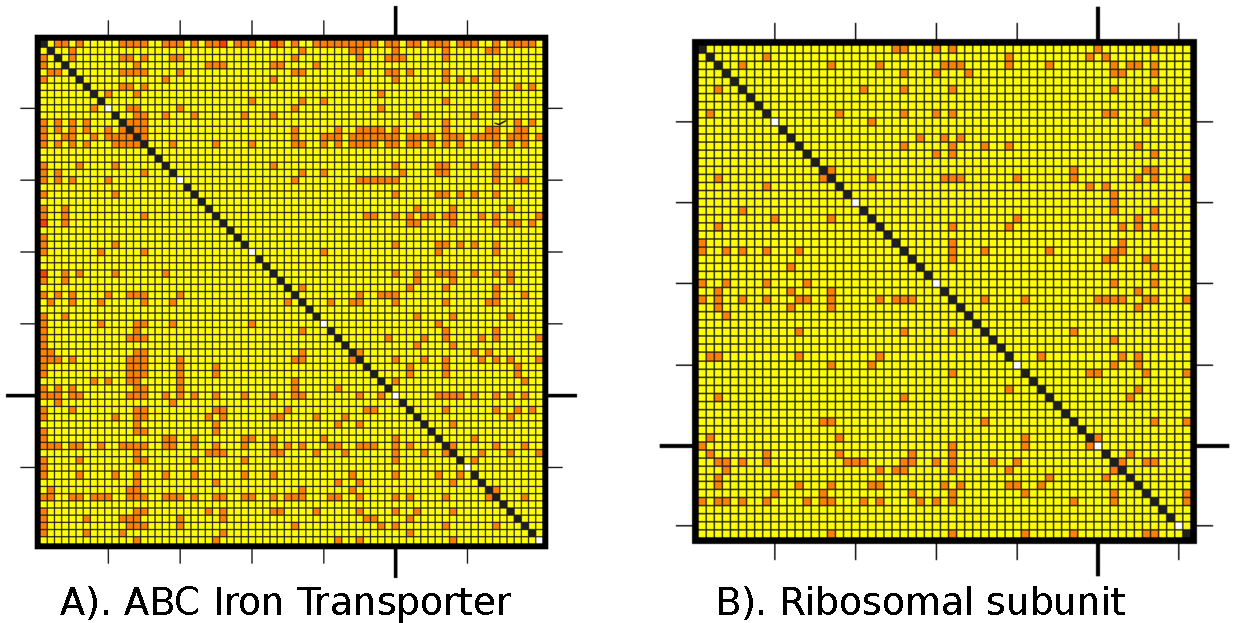
\includegraphics{Figures/Fcylindrus/matrices.pdf}
\caption{Incompatibility score matrices computed for A). The ABC iron Transporter and B). The Large Ribosomal Subunit.
Yellow boxes indicate two informative sites are compatible, and darker boxes indicate the two sites are incompatible.
The presence of incompatible sites in the alignments is suggestive of recombination.\label{fig:FC_Res_2}}
\end{figure}

\begin{table}
\centering
\caption{PHI-Score and Neighbor Similarity Scores of the PCR amplified sequences for three different window sizes.}
\begin{tabular}{ |P{2cm}|P{2cm}|P{2cm}|P{2cm}|P{2cm}|P{2cm}| }
 \hline
 Sequences & Window Size & PHI Score & P-Value & NSS & NSS P-Value \\
 \hline
 FeABC & 100 & 0.0930 & 0.0000405 & 0.81056 & 0.005 \\
 FeABC & 50 & 0.0955 & 0.0041100 & 0.81056 & 0.004 \\
 FeABC & 10 & 0.0870 & 0.0814000 & 0.81056 & 0.006 \\
 Fcl10 & 100 & 0.0930 & 4.0500000 & 0.81056 & 0.005 \\
 Fcl10 & 50 & 0.0385 & 0.0184000 & 0.88306 & 0.342 \\
 Fcl10 & 10 & 0.0500 & 0.2650000 & 0.88306 & 0.338 \\
 \hline
\end{tabular}
\label{table:Phitable}
\end{table}

\subsubsection{Comparative analysis of phylogenetic networks}

Figure \ref{fig:asexnet}. Shows an example network generated from sequences produced by the population genetics simulation scenario, in which individuals reproduced by asexual (clonal) reproduction.
This network is clearly characterized by two distinct clades, separated by long branches.

\begin{figure}
\centering
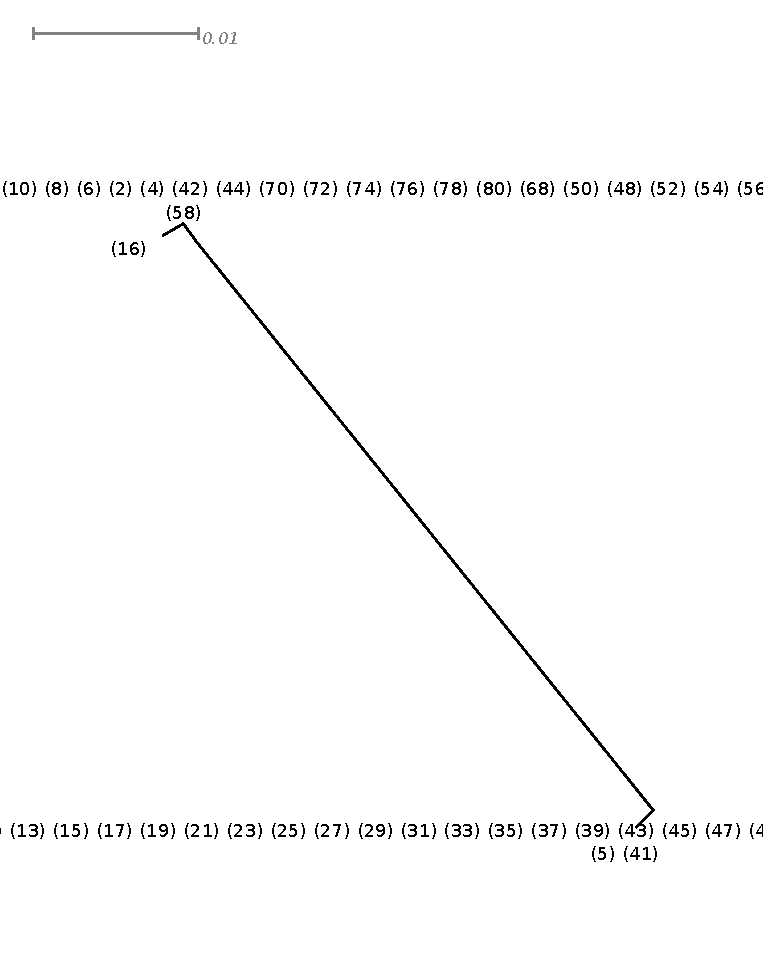
\includegraphics[width=\textwidth,keepaspectratio]{Figures/Fcylindrus/Asexual_randomSub}
\caption{Network of simulated allelic pairs, evolved under an asexual reproduction scheme.
The first copies of each allelic pair form a clade, and the second copies of each allelic pair form a clade.
This is because there is no recombination during gamete formation, as with clonal reproduction, offspring are clones of their parent.\label{fig:asexnet}}
\end{figure}

If \textit{F. cylindrus} has a history of asexual reproduction and ancient allelic divergence, then it is expected that the networks calculated for the PCR amplified sequences of the ABC Iron Transporter and the Large Ribosomal Subunit will have a similar structure to that of the network in Figure \ref{fig:asexnet}.

\begin{figure}
\centering
\subfigure[ABC Iron Transporter]{
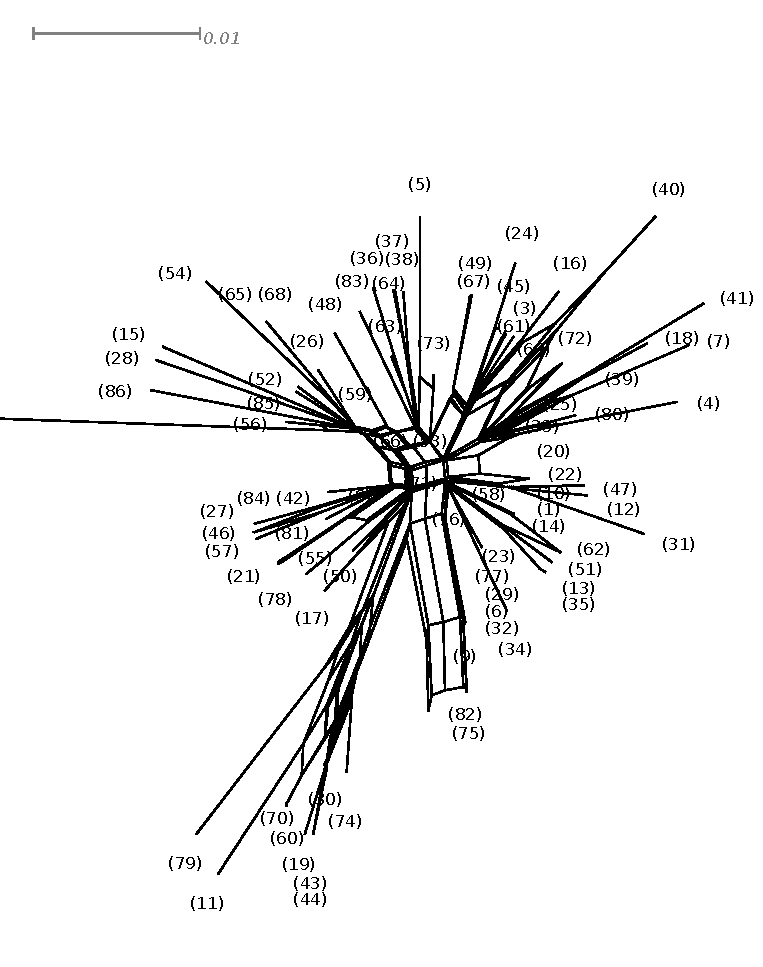
\includegraphics[width=0.5\textwidth]{Figures/Fcylindrus/3rd_Codon_Position_FC_ABC_IronTransporter}
}\\
\subfigure[Large Ribosomal Subunit]{
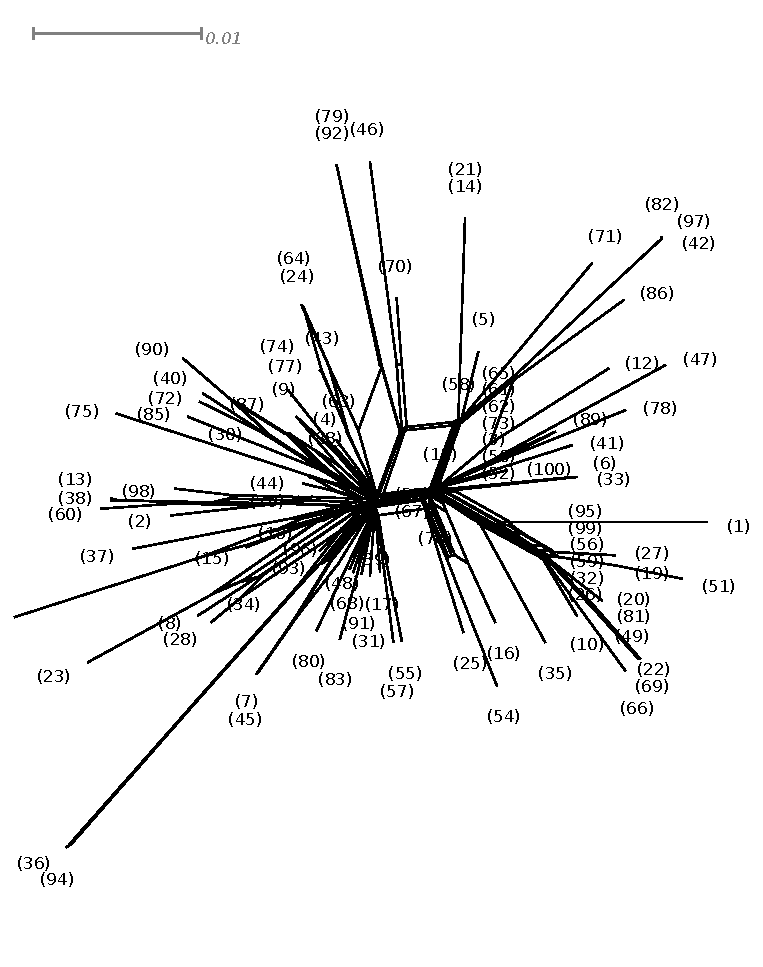
\includegraphics[width=0.5\textwidth]{Figures/Fcylindrus/3rd_Codon_Position_Fcl}
}
\caption{Split Networks of the ABC Iron Transporter and Ribosomal Subunit sequences have average branch lengths close to $10^{-2}$ and contain $~225$ splits. \label{fig:realnets}}
\end{figure}

Panels a and b in Figure \ref{fig:realnets} show the phylogenetic networks calculated for the PCR amplified sequences of the ABC Iron Transporter (a), and the Large Ribosomal Subunit (b).
These two networks are clearly different qualitatively to the kind of network in Figure \ref{fig:asexnet} that would be expected if \textit{F. cylindrus} had a history of asexual reproduction without meiotic recombination.
They do not show a clear partition between two clades or clusters, instead they have average branch lengths of around $0.1$, and contain around $255$ splits. 

\begin{figure}
\centering
\subfigure[The effect of $\theta$ on network branch lengths]{
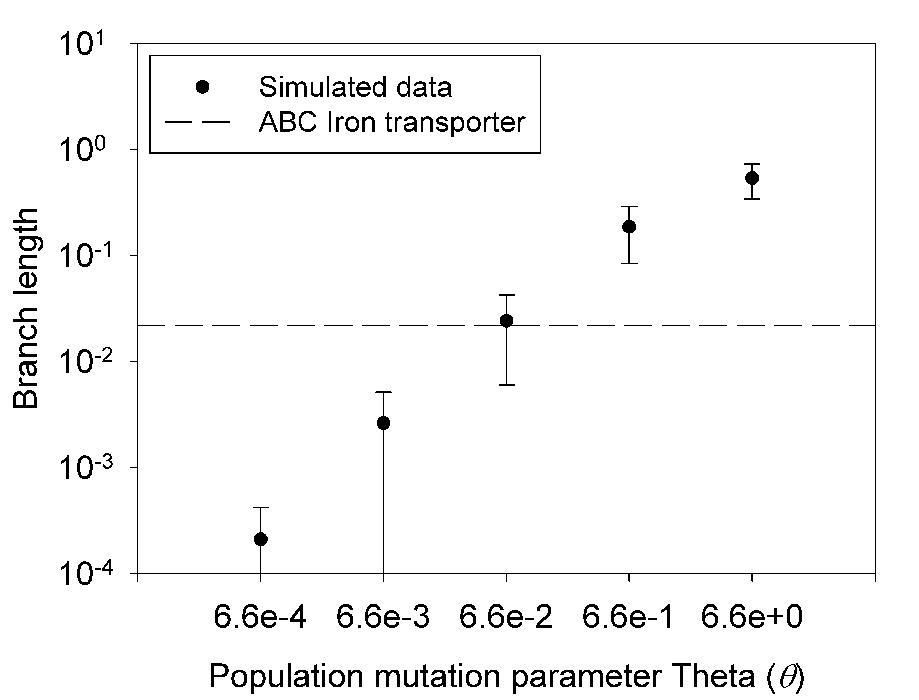
\includegraphics[width=0.8\textwidth]{Figures/Fcylindrus/branchlengths}
}\\
\subfigure[The effect of recombination rate on splits]{
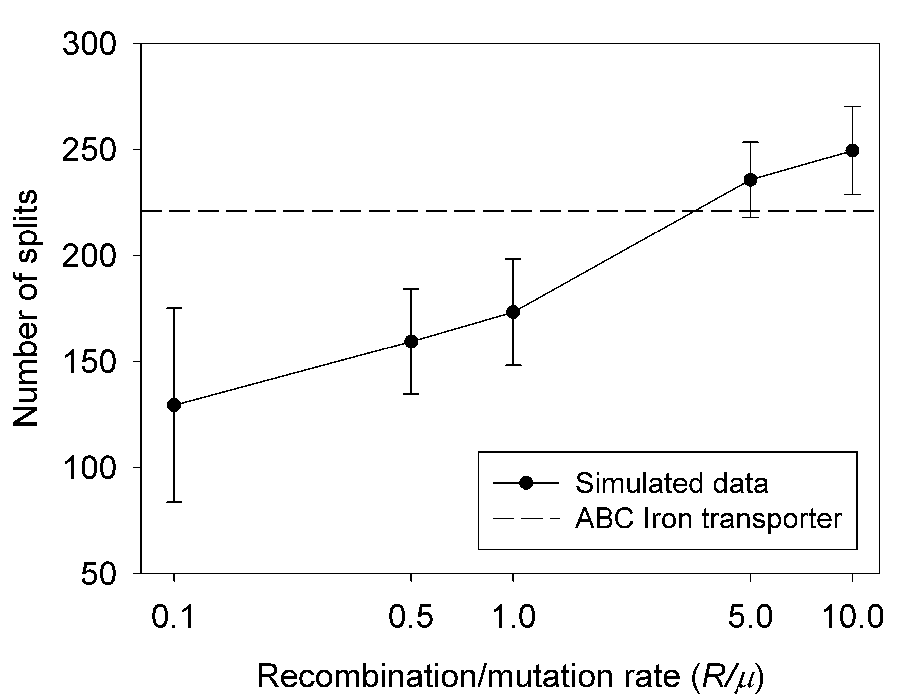
\includegraphics[width=0.8\textwidth]{Figures/Fcylindrus/splitsrmu}
}
\caption{Quantifying the branch lengths and number of splits in networks produced from simulations with varying levels of recombination and values of $\theta$.
Larger values of $\theta$ cause longer branches (a), and higher recombination rates result in more splits (b).\label{fig:relgraphs}}
\end{figure}

Panel a of Figure \ref{fig:relgraphs}, demonstrates the effect of increasing or decreasing $\theta$ in population genetic simulations, on the resulting sequences, and thus the networks produced:
The average branch lengths in networks, is positively related to the $\theta$ parameter set in the simulation.

\begin{figure}
\centering
\subfigure[$\theta = 0.66$]{
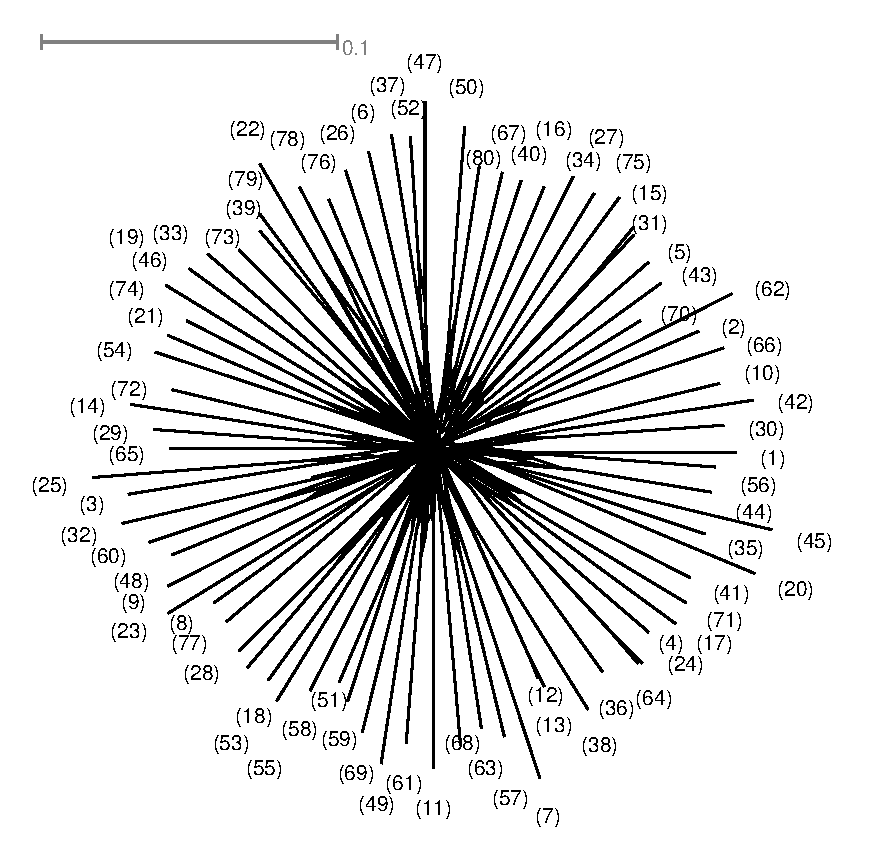
\includegraphics[width=0.5\textwidth]{Figures/Fcylindrus/Theta0_66Net}
}
\subfigure[$\theta = 0.066$]{
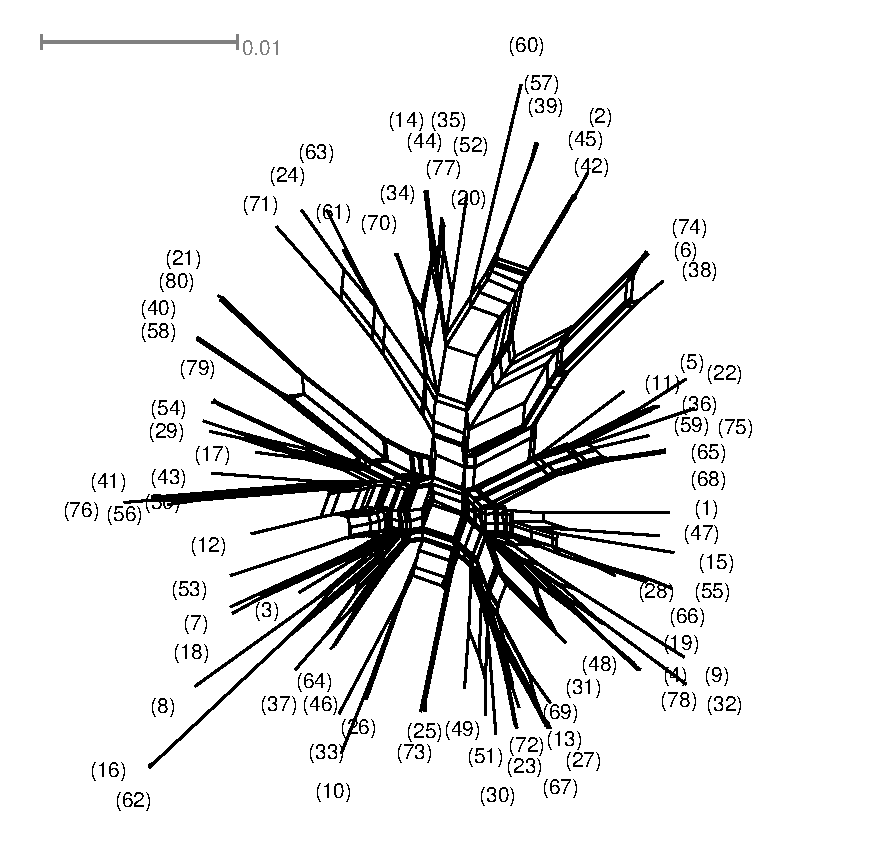
\includegraphics[width=0.5\textwidth]{Figures/Fcylindrus/Theta0_066Net}
}
\subfigure[$\theta = 0.0066$]{
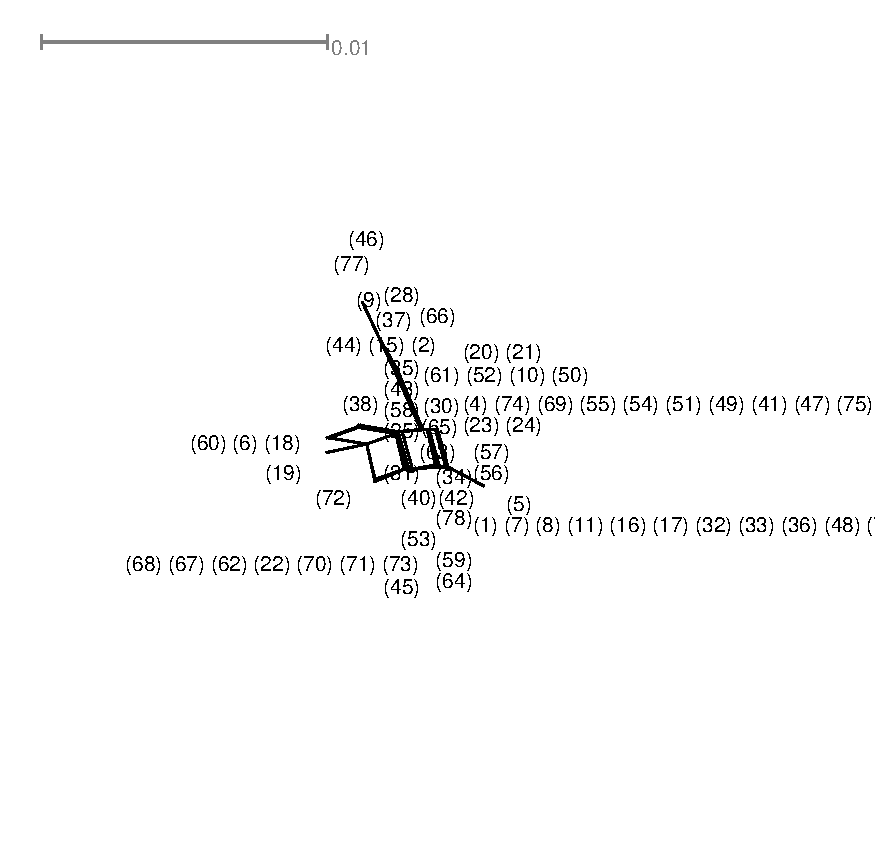
\includegraphics[width=0.5\textwidth]{Figures/Fcylindrus/Theta0_0066Net}
}
\caption{Networks computed from simulations with three different values of $\theta$.
Larger values of $\theta$ result in longer outer branches of networks.\label{fig:blnets}}
\end{figure}

Figure \ref{fig:blnets} presents this relationship qualitatively with the networks produced by Splitstree.
From figures \ref{fig:relgraphs} and \ref{fig:blnets} it can be seen that the networks best matching the real sequence networks (figure \ref{fig:realnets}) in terms of branch lengths, are those produced by simulations where $\theta = 0.066$, which is close to the value which LAMARC has estimated. 

Panel b of figure \ref{fig:relgraphs} demonstrates the effect of varying the recombination rate relative to the mutation rate in population genetic simulations, on the sequences and networks produced: The number of splits in networks is positively related to the recombination rate, relative to the mutation rate. This relationship is shown qualitatively in the networks drawn in figure \ref{fig:splitnets}.

\begin{figure}
\begin{center}
\subfigure[$R/\mu=1$]{
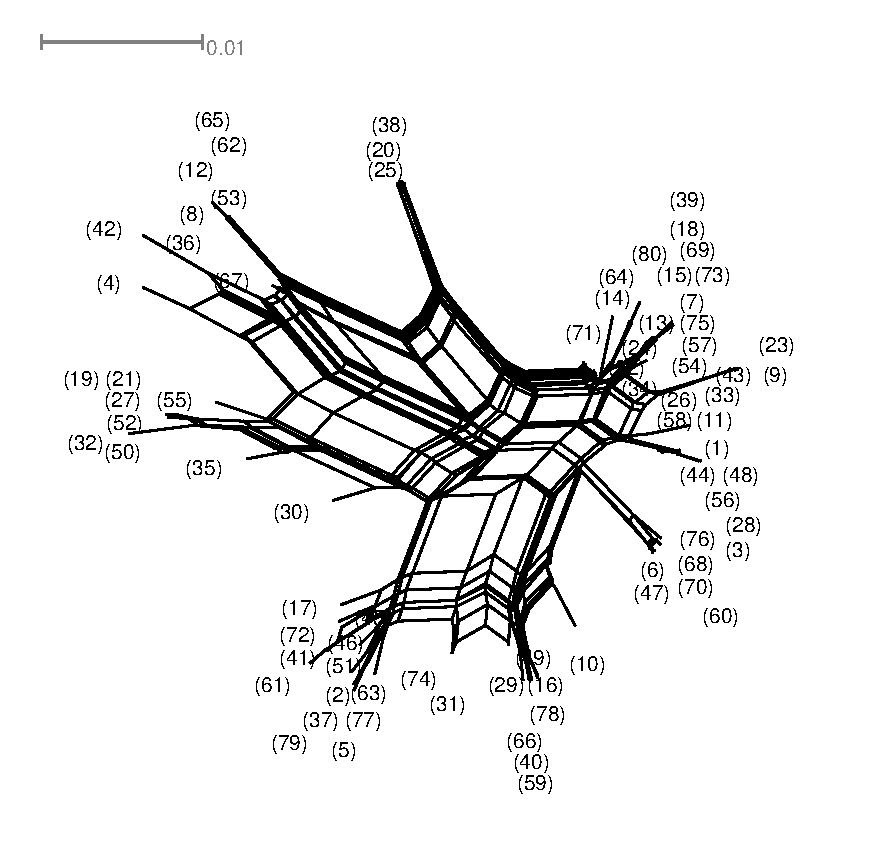
\includegraphics[width=0.5\textwidth]{Figures/Fcylindrus/rmuNet}
}
\subfigure[$R/\mu=5$]{
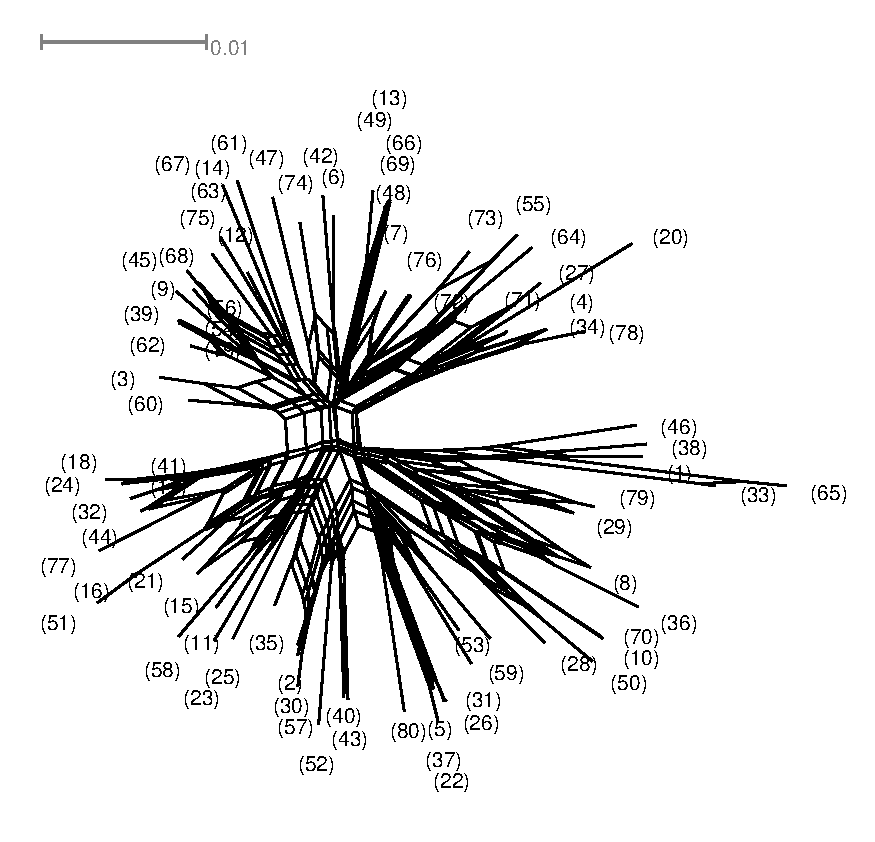
\includegraphics[width=0.5\textwidth]{Figures/Fcylindrus/rmu5Net}
}
\subfigure[$R/\mu=10$]{
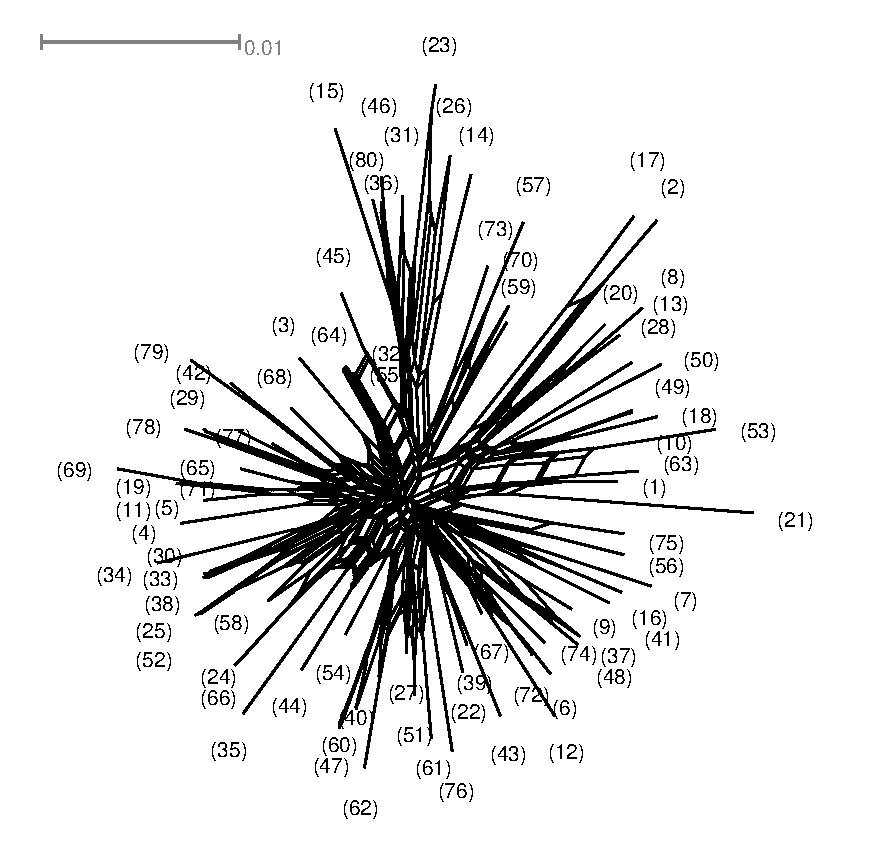
\includegraphics[width=0.5\textwidth]{Figures/Fcylindrus/rmu10Net}
}
\caption{Networks computed from simulations with three different levels of recombination, relative to the mutation rate $\mu$.
Larger values of $R$ result in more splits in networks.\label{fig:splitnets}}
\end{center}
\end{figure}




